\section*{Latencies Reference}
\FloatBarrier
\begin{table}[]
    \centering
    \resizebox{\textwidth}{!}{%
    \begin{tabular}{lllll}
    \hline
    \rowcolor[HTML]{C0C0C0} 
    \multicolumn{1}{c}{\cellcolor[HTML]{C0C0C0}\textbf{Operation}}     & \multicolumn{3}{c}{\cellcolor[HTML]{C0C0C0}\textbf{Latency}}               & \multicolumn{1}{c}{\cellcolor[HTML]{C0C0C0}\textbf{Notes}} \\ \hline
    \rowcolor[HTML]{C0C0C0} 
                                                                       & \textit{\textbf{nano}} & \textit{\textbf{micro}} & \textit{\textbf{milli}} &                                                            \\
    \textit{L1 cache reference}                                        & 0.5                    & 0.000500000             & 0.000000500             & 14 \textbackslash{}times L1 cache                          \\
    \textit{Branch mispredict}                                         & 5                      & 0.005000000             & 0.000005000             &                                                            \\
    \textit{L2 cache reference}                                        & 7                      & 0.007000000             & 0.000007000             &                                                            \\
    \textit{Mutex lock/unlock}                                         & 25                     & 0.025000000             & 0.000025000             &                                                            \\
    \textit{Main Memory Reference}                                     & 100                    & 0.100000000             & 0.000100000             & 20 times L2 cache. 200x L1                                 \\
    \textit{Compress 1K bytes with Zippy}                              & 3000                   & 3.000000000             & 0.003000000             &                                                            \\
    \textit{Send 1K bytes over 1 Gbps network}                         & 10000                  & 10.000000000            & 0.010000000             &                                                            \\
    \textit{Read 4K randomly from SSD*}                                & 150000                 & 150.000000000           & 0.150000000             & $\sim$1GB/sec SSD                                          \\
    \textit{Round trip within same datacenter}                         & 500000                 & 500.000000000           & 0.500000000             &                                                            \\
    \textit{Read 1 MB sequentially from SSD*}                          & 1000000                & 1000.000000000          & 1.000000000             & $\sim$1GB/sec SSD, 4X memory                               \\
    \textit{Disk seek}                                                 & 10000000               & 10000.000000000         & 10.000000000            & 20x datacenter roundtrip                                   \\
    \textit{Read 1 MB sequentially from disk}                          & 20000000               & 20000.000000000         & 20.000000000            & 80x memory, 20X SSD                                        \\
    \textit{Send packet CA-\textgreater{}Netherlands-\textgreater{}CA} & 150000000              & 150000.000000000        & 150.000000000           &                                                           
    \end{tabular}%
    }
    \caption{Latency Comparison Numbers ($\sim$2012). Credit to \url{https://gist.github.com/jboner/2841832}}
    \label{tab:refernce_latencies}
\end{table}
\FloatBarrier


\begin{figure}
	\centering
	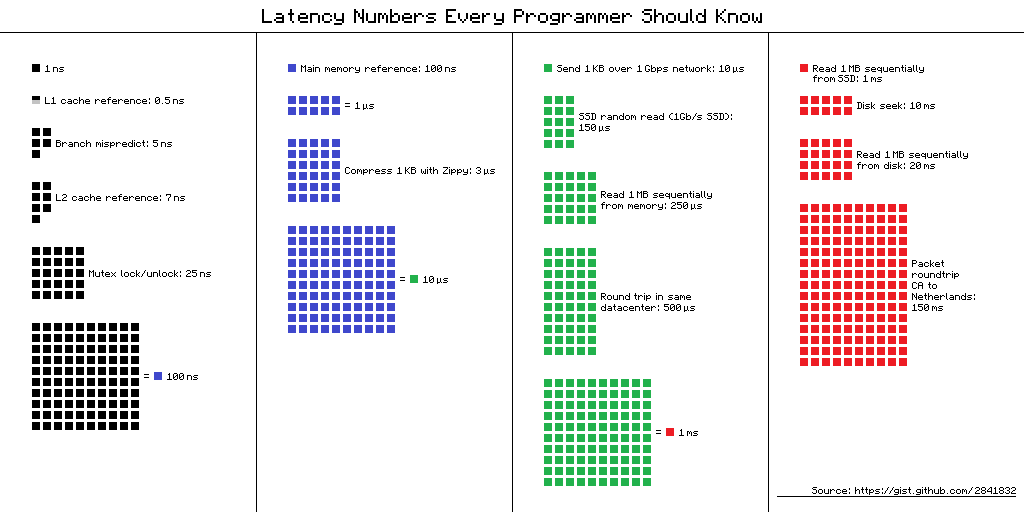
\includegraphics[width=\textwidth]{sources/appendices/images/latencies-refernece.png}
	\caption[]{Humanized visualization of the data in Table 
    \ref{tab:refernce_latencies}}.
	\label{fig:refernce_latencies}
\end{figure}

\FloatBarrier
